\chapter{\MakeUppercase{Project Implementation}}
\section{Implementation Overview}
The project is implemented in Python. The file \verb|environment.py| defines the disaster \ac{dtn} testbed, simulation constants, node creation, message generation, mobility update, contact detection, delivery checking, expiration, and metric computation. The file \verb|message.py| defines message identity, source, destination, creation time, critical flag, hop count, and copy count. The file \verb|node.py| defines node identity, role, mobility properties, location, and buffer.

The routing implementations are placed inside the \verb|routing| package. The baselines are implemented in \verb|routing/epidemic.py| and \verb|routing/spray.py|. The proposed protocol is implemented in \verb|routing/spatio_semantic.py|. The experiment runner in \verb|main.py| executes every protocol across all traffic levels and writes aggregate outputs to the \verb|plots| directory.

\section{Code Structure and Execution Flow}
The implementation follows the same separation of concerns described in the design chapter. The environment acts as the orchestration layer. It initializes nodes, advances time, invokes the selected routing module during contacts, and records outcome statistics. This keeps the experiment control logic in one place and allows the routing files to focus only on forwarding behavior.

The execution flow begins in \verb|main.py|, which defines the protocol list and traffic scenarios to be evaluated. For each combination, the simulator is run repeatedly and the resulting metrics are accumulated. Once all repetitions are complete, the average values are written to protocol-specific \ac{csv} files. This makes the data pipeline straightforward: experiment execution produces files in the \verb|plots| directory, and the dashboard reads those same files for visualization.

\section{Environment Implementation}
The environment creates four node classes:

\begin{itemize}
	\item 35 civilians with slow movement.
	\item 8 responders with medium movement.
	\item 3 static shelters clustered in one region.
	\item 5 drones with high movement speed.
\end{itemize}

At every time step, the environment probabilistically generates messages, moves nodes, detects contacts, invokes router exchanges, checks deliveries, and removes expired messages. This implementation gives all protocols the same external conditions and isolates differences to their routing decisions.

The environment also acts as the central accounting module. It tracks the number of generated messages, delivered messages, critical deliveries, message delays, transmissions, and buffer drops. Placing these counters inside the environment rather than inside individual routers ensures that the performance metrics are computed consistently. Each router may decide differently, but all routers are judged by the same bookkeeping rules.

\section{Routing Baseline Implementation}
The Epidemic router clones messages to any encountered node that lacks the message. It increments the transmission counter for every successful transfer and increments the drop counter when the receiver buffer is full.

The Spray and Wait router uses message copy counts. When a sender has more than one copy, it gives one copy to a receiver that does not already hold the message. When a message has only one copy, it is forwarded only to the destination. This design reduces unnecessary replication but can slow delivery.

These baseline implementations are intentionally simple. Their role in the codebase is not to reproduce every variant from the literature but to provide clear reference behaviors. Epidemic represents unrestricted replication, while Spray and Wait represents strict replica control. Because both baselines are compact and interpretable, the effect of the proposed router can be understood more clearly in both code and results.

\section{Spatio-Semantic Router Implementation}
The proposed router maintains two tracking tables on nodes:

\begin{itemize}
	\item Encounter table: records decayed contact frequency with other nodes.
	\item Zone table: records decayed visit frequency for spatial zones.
\end{itemize}

The router updates these tables during exchanges. It then computes the utility of the sender and receiver relative to the message destination. If the receiver is the destination, delivery is always attempted. Otherwise, the protocol uses message priority and copy count to decide whether to spray, utility-forward, or wait.

In implementation terms, the router behaves as a contact-time decision engine. It reads the sender state, receiver state, and message state at the moment of encounter. From that information it derives utility scores and applies threshold rules that determine whether the message should be transferred and how many copies should move. This design keeps the forwarding logic explicit and makes it easier to relate code behavior to the algorithm presented in the thesis.

\section{Critical Buffer Reserve}
The implementation reserves 35 percent of the buffer for critical messages. Non-critical messages can only occupy the non-reserved portion. Critical messages can use any available slot and can evict a non-critical message if necessary. This prevents non-critical traffic from consuming all storage during high-load conditions.

The reserve policy is one of the clearest examples of implementation following the thesis objective. Instead of handling priority only in abstract utility scores, the code enforces priority at insertion time. This matters because a router can select a good relay correctly and still fail to preserve an urgent message if the receiver buffer is already filled with less important traffic. The eviction rule therefore translates the conceptual importance of critical traffic into an actual storage guarantee.

\section{Result and Visualization Implementation}
The file \verb|dashboard.py| loads the three result files:

\begin{itemize}
	\item \verb|plots/epidemic_results.csv|
	\item \verb|plots/spray_results.csv|
	\item \verb|plots/spatio_semantic_results.csv|
\end{itemize}

The dashboard provides trend graphs, radar charts, raw data tables, and a launch button for the visual simulation. The file \verb|modern_multi_demo.py| displays a full-screen three-panel comparison of Epidemic, Spray and Wait, and Spatio-Semantic routing.

This implementation layer is useful beyond presentation. The dashboard creates a direct bridge between the experiment code and the analytical discussion of the thesis. Because the plots are produced from the same stored metrics used in the tables, visual inspection and tabular analysis remain consistent. The live visual comparison also helps explain why a protocol behaves as observed, especially when congestion, clustering, and mobile relays create differences that are easier to understand visually than numerically.

\section{Implementation Choices for Maintainability}
Several implementation choices were made to keep the project maintainable. Protocol logic is separated from environment logic so that algorithm changes do not require rewriting message generation, movement, or metric collection. Data is exported in a simple format so that the analysis layer remains independent of the simulation engine. These decisions reduce coupling and make the code easier to verify and extend.

Maintainability also matters for thesis credibility. When a project contains several interacting modules, unclear code structure can make it difficult to explain how results were produced. By organizing the simulator into small files with distinct responsibilities, the implementation supports both repeatable experimentation and clear academic reporting. This is especially valuable when the thesis compares multiple routing strategies under the same framework.

\section{Metric Export Workflow}
After each experiment set is completed, the aggregated metrics are written to the \verb|plots| directory as protocol-specific result files. This export step is intentionally simple because the same files are later consumed by the dashboard and referenced by the thesis tables. A clean metric-export workflow reduces the chance of mismatch between the simulation output and the presented analysis.

This workflow also improves repeatability. If a parameter is changed and the experiments are rerun, the updated \ac{csv} outputs provide a clear record of the new results without requiring manual transcription. In practice, this allows the project to support an efficient cycle of implementation, execution, inspection, and revision, which is important when comparing several routing strategies across multiple traffic conditions.

\begin{figure}[h!]
    \centering
    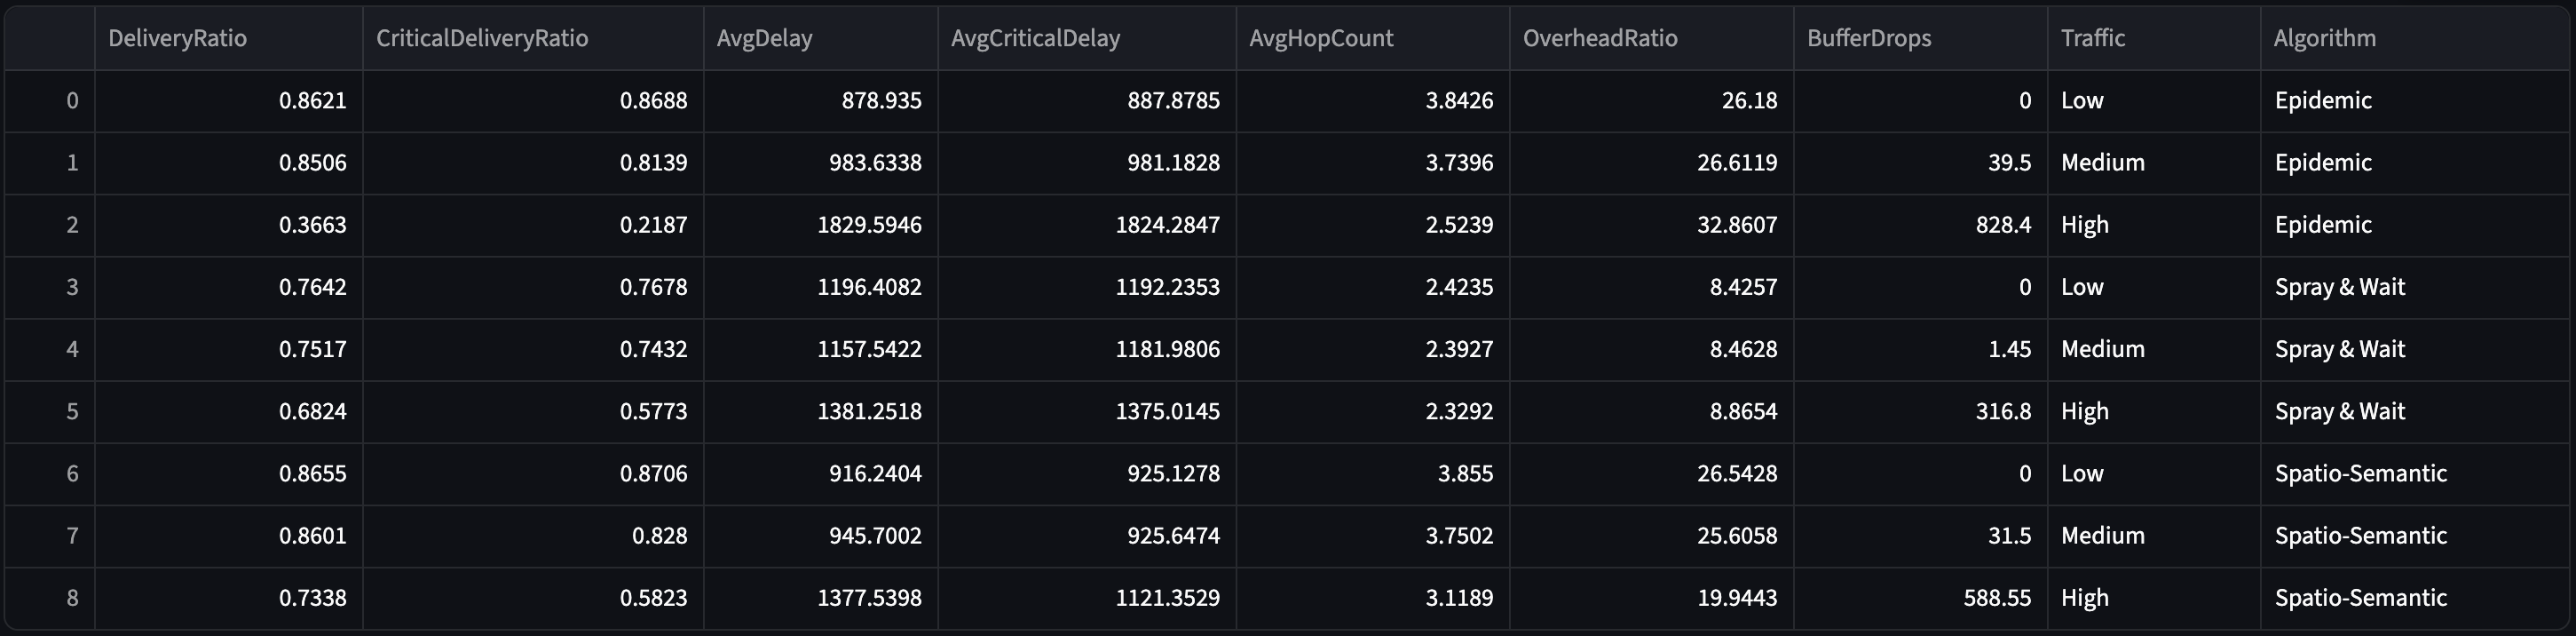
\includegraphics[width=0.85\textwidth]{images/raw-data.png}
    \caption{Raw aggregated simulation results in the dashboard}
    \label{fig:raw_data_placeholder}
\end{figure}
